%---------------------------------------------------------------------------
\addtocounter{framenumber}{-1}
\begin{frame}[t]
\end{frame}
%---------------------------------------------------------------------------
\addtocounter{framenumber}{-1}
\begin{frame}[t]
\frametitle{Rb-VMS Summary}
% \begin{table}[h]
% \centering
% \begin{tabular}{|c|c|c|c|c|}
% \hline
% & Sgs space & Sgs dynamics                         &  Advection velocity ($\mathbf{a}$)  \\
% \hline
% 1&ASGS      & Static  ($\tilde{\mathbf{u}}=f(\mathbf{R}_m)$) &  Linear ($\mathbf{a}=\mathbf{u}_h$) \\
% 2&ASGS      & Dynamic ($\tilde{\mathbf{u}}=f(\mathbf{R}_m,\partial_t\tilde{\mathbf{u}})$)&  Linear ($\mathbf{a}=\mathbf{u}_h$) \\
% 3&ASGS      & Dynamic ($\tilde{\mathbf{u}}=f(\mathbf{R}_m,\partial_t\tilde{\mathbf{u}})$)&  Nonlinear ($\mathbf{a}=\mathbf{u}_h+\tilde{\mathbf{u}}$) \\
% \hline
% 4&OSS      & Static  ($\tilde{\mathbf{u}}=f(\mathbf{R}_m)$)  &  Linear ($\mathbf{a}=\mathbf{u}_h$) \\
% 5&OSS      & Dynamic ($\tilde{\mathbf{u}}=f(\mathbf{R}_m,\partial_t\tilde{\mathbf{u}})$)&  Linear ($\mathbf{a}=\mathbf{u}_h$) \\
% 6&OSS      & Dynamic ($\tilde{\mathbf{u}}=f(\mathbf{R}_m,\partial_t\tilde{\mathbf{u}})$)&  Nonlinear ($\mathbf{a}=\mathbf{u}_h+\tilde{\mathbf{u}}$) \\
% \hline
% \end{tabular}
% \end{table}

\begin{table}[h]
\centering
\begin{tabular}{|c|c|c|c|c|}
\hline
& Sgs space & Sgs dynamics  &  Advection\\
\hline
1&ASGS      & Static  &  Linear    \\
2&ASGS      & Dynamic &  Linear    \\
3&ASGS      & Dynamic &  Nonlinear \\
\hline
4&OSS      & Static  &  Linear   \\
5&OSS      & Dynamic &  Linear   \\
6&OSS      & Dynamic &  Nonlinear \\
\hline
\end{tabular}
\end{table}
\vskip 0.5 cm
\begin{itemize}
\item[1] It is the most standard method (SUPG for linear elements) up to the choice of the
stabilization parameters. Unknown stability properties.
%\item[2] Proven stability for the linearized problem (Oseen) without $\delta t$ restrictions (Codina et al. 2006)
\item[4] Strictly point-wise positive for linear elements (no backscatter).
\item[5] Convergent to weak solutions of NS equations (Badia \& Gutierrez 2012).
\end{itemize}
\end{frame}
%---------------------------------------------------------------------------
\addtocounter{framenumber}{-1}
\begin{frame}[t]
\frametitle{Energy statements}
\begin{overlayarea}{\textwidth}{0.25\textheight}
\textbf{FE counterpart:}
\vspace*{-0.3cm}
\only<1>{
\begin{align*}
&B\left(\left(\mathbf{u}_h,p_h\right);\left(\widetilde{\mathbf{u}},\widetilde{p}\right);\left(\mathbf{u}_h,p_h\right)\right)=L\left(\mathbf{u}_h,p_h\right)
\end{align*}}
\only<2->{
\begin{align*}
&\alert<3>{\frac{1}{2}d_t\|\u_h\|^2}+\alert<4>{\nu\|\nabla\u_h\|^2}+\alert<5>{b(\a,\u_h,\u_h)}\\
&\alert<7>{+\left( \partial _{t}\widetilde{\u},\u_{h}\right)
+\left( \mathcal{L}^{\ast }_a(\u_{h},p_h),\widetilde{\u}\right)
-\left( \mathbf{\nabla }\cdot \u_{h},\widetilde{p}\right)}
=\alert<8>{\left\langle \mathbf{f},\u_{h}\right\rangle}
\end{align*}}
\end{overlayarea}
\begin{overlayarea}{\textwidth}{0.25\textheight}
\textbf{SGS counterpart:}
\vspace*{-0.3cm}
\only<1>{
\begin{align*}
&B\left(\left(\widetilde{\mathbf{u}},\widetilde{p}\right);\left(\mathbf{u}_h,p_h\right);\left(\widetilde{\mathbf{u}},\widetilde{p}\right)\right)=L\left(\widetilde{\mathbf{u}},\widetilde{p}\right)
\end{align*}}
\only<2->{
\begin{align*}
&\alert<3>{\frac{1}{2}d_t\|\widetilde{\u}\|^2}\alert<6>{+\tau_m^{-1}\|\widetilde{\u}\|^2+\tau_c^{-1}\|\widetilde{p}\|^2}\\
&\alert<7>{+\left( \mathcal{P}(\partial _{t}\u_{h}),\widetilde{\u}\right)
+\left( \mathcal{P}(\mathcal{L}^{\ast }_a(\u_{h},p_h)),\widetilde{\u}\right)
-\left( \mathcal{P}(\mathbf{\nabla }\cdot \u_{h}),\widetilde{p}\right)}
=\alert<8>{\left\langle \mathcal{P}(\mathbf{f}),\widetilde{\u}\right\rangle}
\end{align*}}
\end{overlayarea}
\begin{overlayarea}{\textwidth}{0.5\textheight}
\textbf{TOTAL:}
\only<9>{\alert<9>{\textbf{ Static subscales}}}
\only<10->{\alert<10->{\textbf{ Dynamic subscales}}}
\only<10>{\alert<10>{\textbf{- ASGS}}}
\only<11>{\alert<11>{\textbf{- OSS}}}
\only<1>{
\begin{align*}
&B\left(\left(\mathbf{u}_h,p_h\right);\left(\widetilde{\mathbf{u}},\widetilde{p}\right);\left(\mathbf{u}_h,p_h\right)\right)\\
+&B\left(\left(\widetilde{\mathbf{u}},\widetilde{p}\right);\left(\mathbf{u}_h,p_h\right);\left(\widetilde{\mathbf{u}},\widetilde{p}\right)\right)=L\left(\mathbf{u}_h,p_h\right)+L\left(\widetilde{\mathbf{u}},\widetilde{p}\right)
\end{align*}}
\only<3-8>{
\begin{align*}
&\alert<3>{\frac{1}{2}d_t\|\u_h\|^2+\frac{1}{2}d_t\|\widetilde{\u}\|^2}
\onslide<4-8>{
\alert<4>{+\nu\|\nabla\u_h\|^2}
\onslide<6-8>{
\alert<6>{+\tau_m^{-1}\|\widetilde{\u}\|^2+\tau_c^{-1}\|\widetilde{p}\|^2}\\
\onslide<7-8>{
&\alert<7>{+\left( \partial _{t}\widetilde{\u},\u_{h}\right)+\left( \mathcal{P}(\partial _{t}\u_{h}),\widetilde{\u}\right)
+\left( \mathcal{L}^{\ast }_a(\u_{h},p_h),\widetilde{\u}\right)+\left( \mathcal{P}(\mathcal{L}^{\ast }_a(\u_{h},p_h)),\widetilde{\u}\right)}\\
&\alert<7>{
-\left( \mathbf{\nabla }\cdot \u_{h},\widetilde{p}\right)
-\left( \mathcal{P}(\mathbf{\nabla }\cdot \u_{h}),\widetilde{p}\right)}
\onslide<8>{
=\alert<8>{\left\langle \mathbf{f},\u_{h}\right\rangle+\left\langle \mathcal{P}(\mathbf{f}),\widetilde{\u}\right\rangle}
}}}}
\end{align*}}
\only<9->{
\begin{align*}
&\only<9,11>{\frac{1}{2}d_t\|\u_h\|^2}
\only<10>{\frac{1}{2}d_t\|\u_h+\widetilde{\u}\|^2}
\onslide<11>{+\frac{1}{2}d_t\|\widetilde{\u}\|^2}
+\nu\|\nabla\u_h\|^2
+\tau_m^{-1}\|\widetilde{\u}\|^2+\tau_c^{-1}\|\widetilde{p}\|^2\\
&\only<9>{\onslide<11>{+\left( \partial _{t}\widetilde{\u},\u_{h}\right)}+\left( \mathcal{P}(\partial _{t}\u_{h}),\widetilde{\u}\right)
+\left( \mathcal{L}^{\ast }_a(\u_{h},p_h),\widetilde{\u}\right)+\left( \mathcal{P}(\mathcal{L}^{\ast }_a(\u_{h},p_h)),\widetilde{\u}\right)}
\only<10,11>{-2\left( \nu\Delta\u_h,\widetilde{\u}\right)}\\
&\onslide<9>{-\left( \mathbf{\nabla }\cdot \u_{h},\widetilde{p}\right)
-\left( \mathcal{P}(\mathbf{\nabla }\cdot \u_{h}),\widetilde{p}\right)}
=\left\langle \mathbf{f},\u_{h}\right\rangle
\only<9,11>{+\left\langle \mathcal{P}(\mathbf{f}),\widetilde{\u}\right\rangle}
\only<10>{+\left\langle \mathbf{f},\widetilde{\u}\right\rangle}
\end{align*}}
\end{overlayarea}

\end{frame}
%---------------------------------------------------------------------------
\addtocounter{framenumber}{-1}
\begin{frame}[t]
\frametitle{Rb-VMS TCF {\small Turbulent Channel Flow}}
\textbf{Reynolds shear stress (models):}
  \vspace*{-0.3cm}
  \begin{figure}
    \centering	
    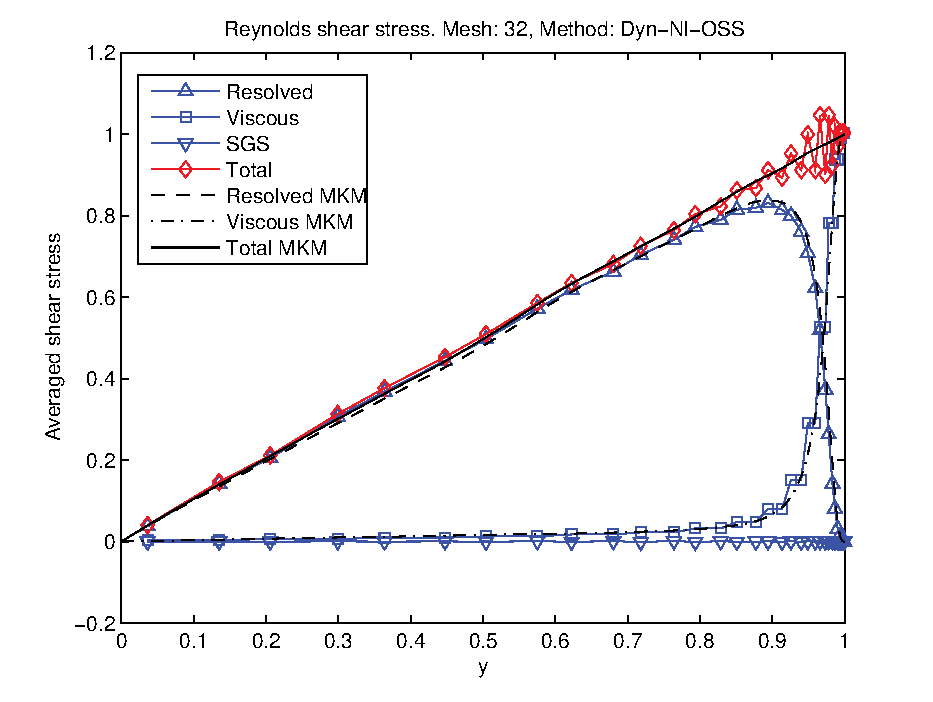
\includegraphics[width=0.7\textwidth]{Figures/Rb_TCF/reystr_395_Dyn_Nl_OSS.pdf}
  \end{figure}
  \vspace*{-0.5cm}
  \begin{overlayarea}{\textwidth}{1.5cm}
 \only<2->{
 \begin{itemize}
  	\item \alert<2>{Almost identical to the DNS}.
  	\only<3->{\item \alert<3>{SGS counterpart does not contribute} to the Reynolds shear stress. }
  \end{itemize}}
  \end{overlayarea}
\end{frame}
%----------------------------------------------------------------------------------------
\addtocounter{framenumber}{-1}
\begin{frame}
 \frametitle{Mixed FE Colliding flow}
 \textbf{Accuracy:} \only<1-2>{Velocity error}\only<3-4>{Pressure error}
   \vspace*{-0.25cm}
 \only<1-3>{
 \begin{figure}
     \centering	
     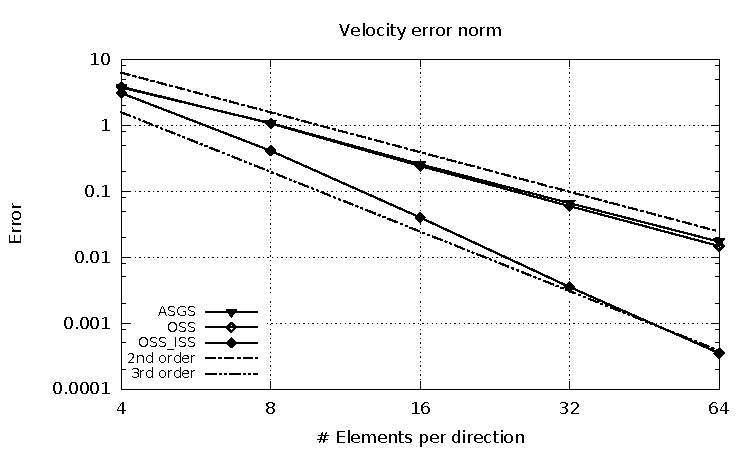
\includegraphics[width=0.8\textwidth]{Figures/colliding_erru.pdf}
   \end{figure}}
\only<4->{
\begin{figure}
    \centering	
    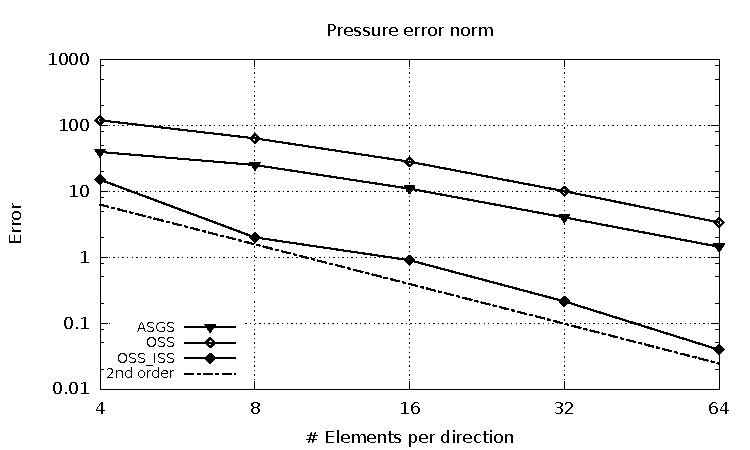
\includegraphics[width=0.8\textwidth]{Figures/colliding_errp.pdf}
  \end{figure}}
 \begin{overlayarea}{\textwidth}{1.5cm}
  \vspace*{-0.5cm}
 \only<2-3>{
 \begin{itemize}
  	\item \alert<2>{2nd order} convergence rate for ASGS and OSS methods.
  	\only<3->{\item \alert<3>{3rd order} convergence rate for OSS-ISS method.}
  \end{itemize}}
   \only<5->{
   \begin{itemize}
    	\item \alert<5>{2nd order} convergence rate for all methods.
    	\only<6->{\item \alert<6>{Best accuracy for OSS-ISS method}.}
    \end{itemize}}
  \end{overlayarea}
\end{frame}
%----------------------------------------------------------------------------------------
\addtocounter{framenumber}{-1}
\begin{frame}
 \frametitle{Mixed FE TGV {\small Taylor-Green Vortex flow}}
 \textbf{Energy dissipation rate (different methods):}
 \vspace*{-0.3cm}
   \begin{figure}
     \centering	
     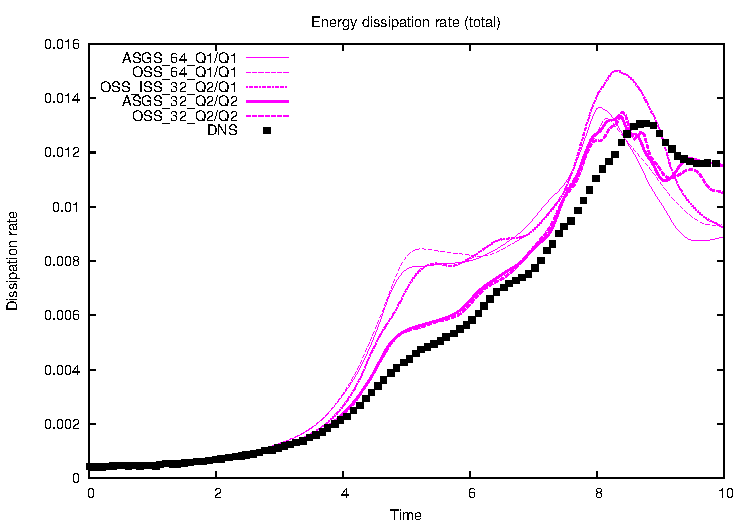
\includegraphics[width=0.65\textwidth]{Figures/oss_64_tot.pdf}
     \vspace*{-0.3cm}
     \caption{Total energy dissipation rate}
   \end{figure}
 \begin{overlayarea}{\textwidth}{1.5cm}
 \only<2->{
 \vspace*{-0.5cm}
 \begin{itemize}
   	\item \alert<2>{Good agreement with the DNS} (coarse mesh).
   	\only<3->{\item \alert<3>{More accurate results with equal-order elements}.}
  \end{itemize}}
  \end{overlayarea}
\end{frame}
%----------------------------------------------------------------------------------------
\addtocounter{framenumber}{-1}
\begin{frame}
 \frametitle{Mixed FE TGV {\small Taylor-Green Vortex flow}}
 \textbf{Energy dissipation rate (refinement OSS-ISS):}
 \vspace*{-0.1cm}
   \begin{figure}
     \centering	
     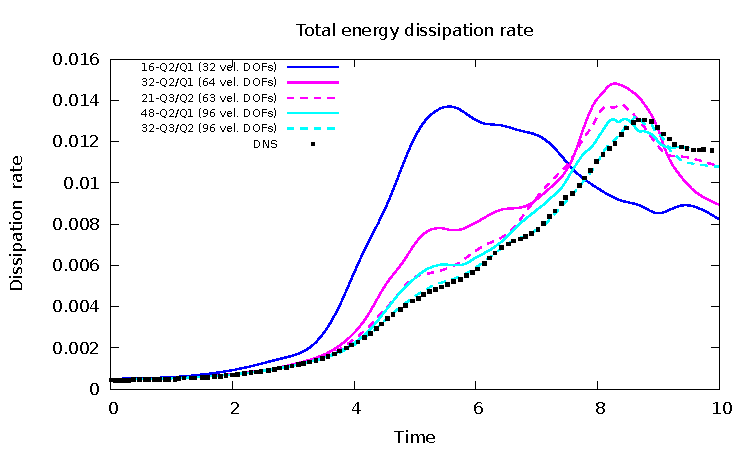
\includegraphics[width=0.75\textwidth]{Figures/TGV_OSS_ISS_refinement_tot.pdf}
     \vspace*{-0.3cm}
     \caption{Total energy dissipation rate}
   \end{figure}
 \begin{overlayarea}{\textwidth}{1.5cm}
 \only<2->{
 \vspace*{-0.5cm}
 \begin{itemize}
   	\item \alert<2>{Good agreement with the DNS}.
   	\only<3->{\item \alert<3>{$ 32^3 $ $ Q3/Q2 $ elements mesh on top of DNS}.}
  \end{itemize}}
  \end{overlayarea}
\end{frame}
%----------------------------------------------------------------------------------------
\addtocounter{framenumber}{-1}
\begin{frame}
\frametitle{SRK 2D Laminar flow around a cylinder}
\textbf{Adaptive time stepping:}
\begin{figure}[h!]
  \centering
  \subfigure[Time step evolution]{\label{fig:IMEX_RK_cyl_adp_dt}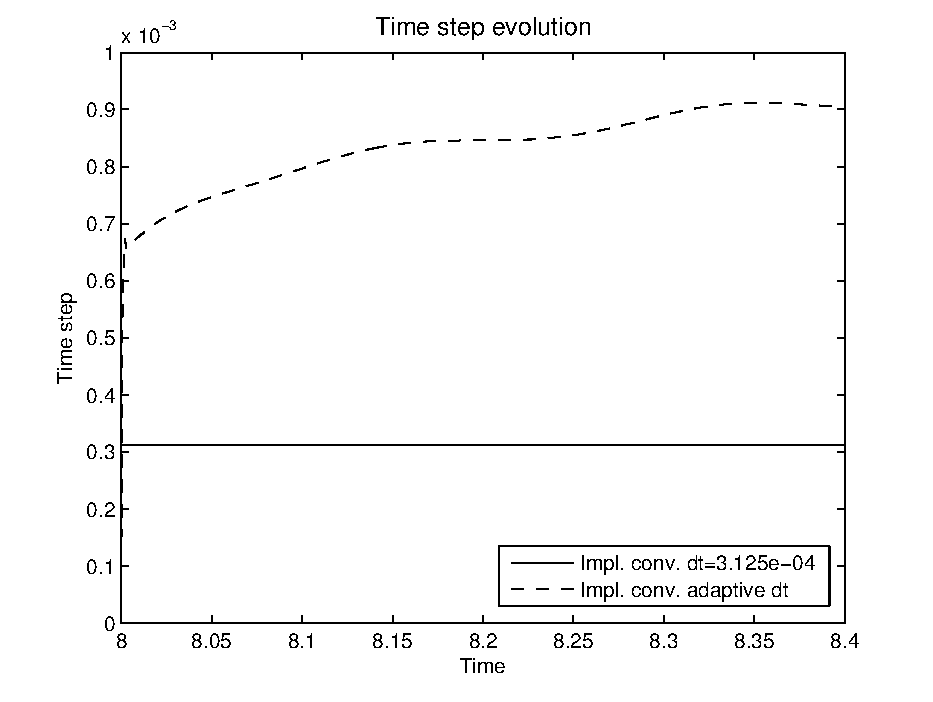
\includegraphics[width=0.49\textwidth]{Figures/time_step}}    
  \subfigure[Lift coefficient (zoom)]{\label{fig:IMEX_RK_cyl_adp_lift}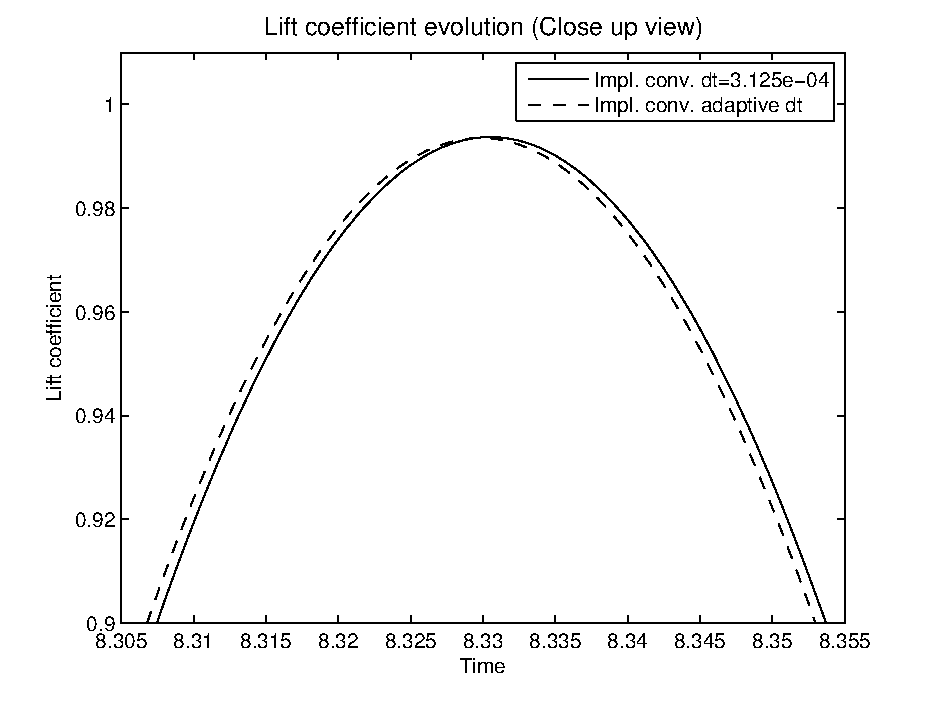
\includegraphics[width=0.49\textwidth]{Figures/lift_close}}
  \caption{Adaptive time stepping.}
  \label{fig:IMEX_RK_cyl_adp}
\end{figure}
\end{frame}